\documentclass{standalone}
\usepackage{tikz}
\usetikzlibrary{patterns, positioning}


\begin{document}
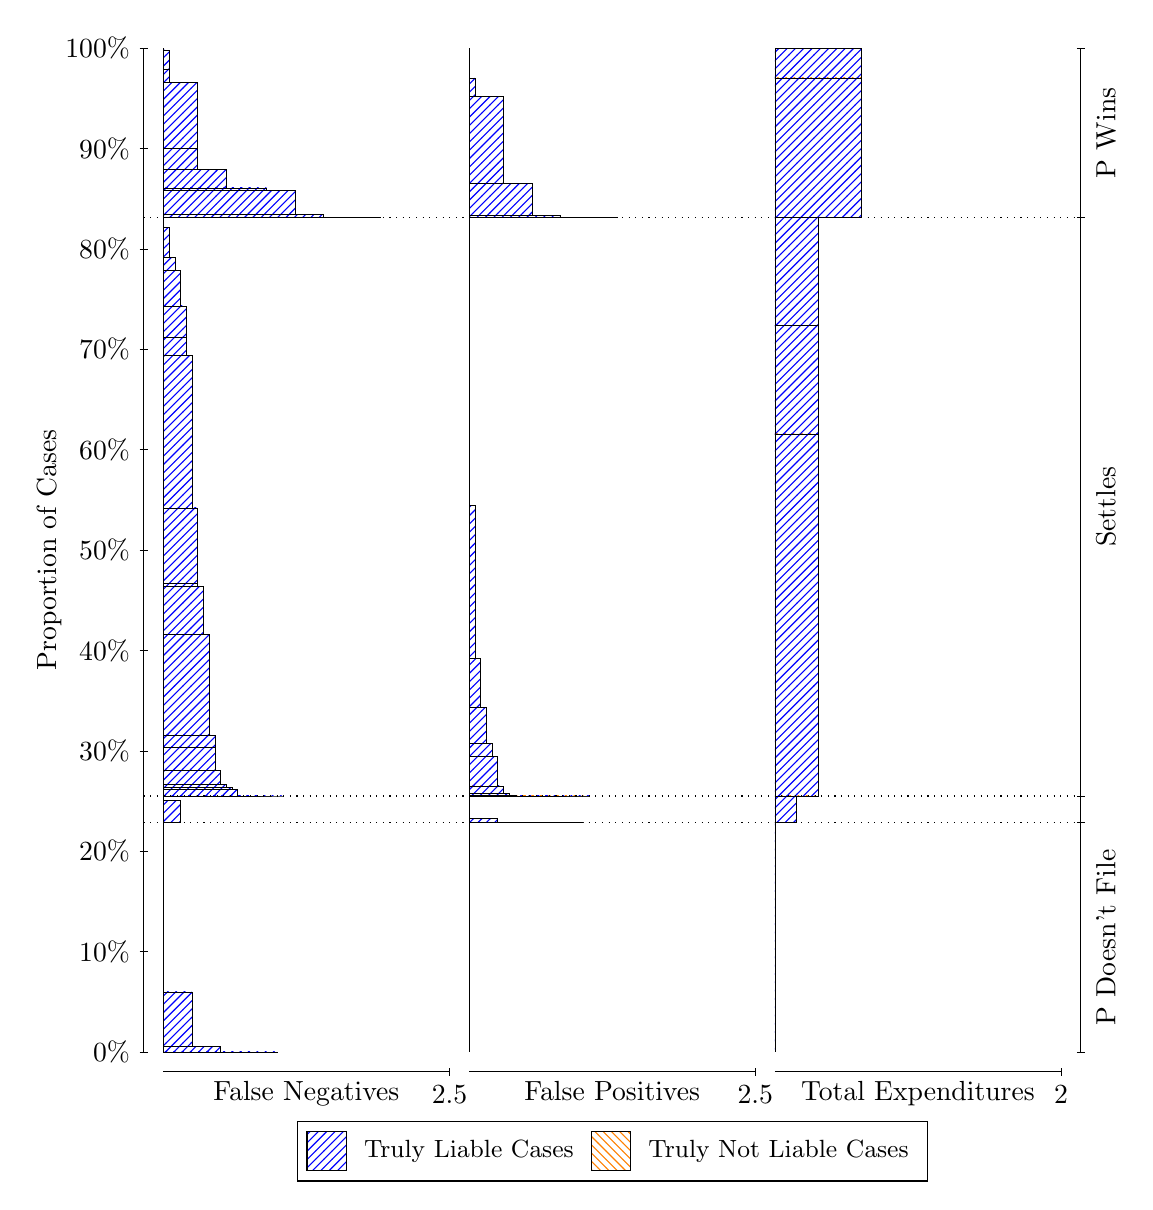
\begin{tikzpicture}
\draw[black, very thin] (1.5,1.75) -- (1.5,14.5);
\node[rotate=90, text=black, anchor=center] at (0.3, 8.125) {Proportion of Cases};
\draw[black, very thin] (1.45,1.75) -- (1.55,1.75);
\node[text=black, anchor=east] at (1.45, 1.75) {0\%};
\draw[black, very thin] (1.45,3.025) -- (1.55,3.025);
\node[text=black, anchor=east] at (1.45, 3.025) {10\%};
\draw[black, very thin] (1.45,4.3) -- (1.55,4.3);
\node[text=black, anchor=east] at (1.45, 4.3) {20\%};
\draw[black, very thin] (1.45,5.575) -- (1.55,5.575);
\node[text=black, anchor=east] at (1.45, 5.575) {30\%};
\draw[black, very thin] (1.45,6.85) -- (1.55,6.85);
\node[text=black, anchor=east] at (1.45, 6.85) {40\%};
\draw[black, very thin] (1.45,8.125) -- (1.55,8.125);
\node[text=black, anchor=east] at (1.45, 8.125) {50\%};
\draw[black, very thin] (1.45,9.4) -- (1.55,9.4);
\node[text=black, anchor=east] at (1.45, 9.4) {60\%};
\draw[black, very thin] (1.45,10.675) -- (1.55,10.675);
\node[text=black, anchor=east] at (1.45, 10.675) {70\%};
\draw[black, very thin] (1.45,11.95) -- (1.55,11.95);
\node[text=black, anchor=east] at (1.45, 11.95) {80\%};
\draw[black, very thin] (1.45,13.225) -- (1.55,13.225);
\node[text=black, anchor=east] at (1.45, 13.225) {90\%};
\draw[black, very thin] (1.45,14.5) -- (1.55,14.5);
\node[text=black, anchor=east] at (1.45, 14.5) {100\%};

\draw[black, very thin] (13.4,1.75) -- (13.4,14.5);
\draw[black, very thin] (13.35,1.75) -- (13.45,1.75);
\node[anchor=west] at (13.35, 1.75) {};
\draw[black, very thin] (13.35,4.6609) -- (13.45,4.6609);
\node[anchor=west] at (13.35, 4.6609) {};
\draw[black, very thin] (13.35,5.001) -- (13.45,5.001);
\node[anchor=west] at (13.35, 5.001) {};
\draw[black, very thin] (13.35,12.346) -- (13.45,12.346);
\node[anchor=west] at (13.35, 12.346) {};
\draw[black, very thin] (13.35,14.5) -- (13.45,14.5);
\node[anchor=west] at (13.35, 14.5) {};

\draw[black, very thin, pattern color=blue, pattern=north east lines] (1.75,1.75) rectangle (3.2033,1.75);
\draw[black, very thin, pattern color=blue, pattern=north east lines] (1.75,1.75) rectangle (2.84,1.7506);
\draw[black, very thin, pattern color=blue, pattern=north east lines] (1.75,1.7506) rectangle (2.4767,1.8208);
\draw[black, very thin, pattern color=blue, pattern=north east lines] (1.75,1.8208) rectangle (2.1133,2.5125);
\draw[black, very thin, pattern color=orange, pattern=north west lines] (1.75,2.5125) rectangle (1.75,2.5125);
\draw[black, very thin, pattern color=blue, pattern=north east lines] (1.75,2.5125) rectangle (1.75,4.6609);
\draw[black, very thin, pattern color=blue, pattern=north east lines] (1.75,4.6609) rectangle (1.968,4.9454);
\draw[black, very thin, pattern color=orange, pattern=north west lines] (1.75,4.9454) rectangle (1.75,4.9454);
\draw[black, very thin, pattern color=blue, pattern=north east lines] (1.75,4.9454) rectangle (1.75,5.001);
\draw[black, very thin, pattern color=blue, pattern=north east lines] (1.75,5.001) rectangle (3.276,5.001);
\draw[black, very thin, pattern color=blue, pattern=north east lines] (1.75,5.001) rectangle (3.1307,5.001);
\draw[black, very thin, pattern color=blue, pattern=north east lines] (1.75,5.001) rectangle (2.9853,5.001);
\draw[black, very thin, pattern color=blue, pattern=north east lines] (1.75,5.001) rectangle (2.9127,5.001);
\draw[black, very thin, pattern color=blue, pattern=north east lines] (1.75,5.001) rectangle (2.84,5.0015);
\draw[black, very thin, pattern color=blue, pattern=north east lines] (1.75,5.0015) rectangle (2.7673,5.0018);
\draw[black, very thin, pattern color=blue, pattern=north east lines] (1.75,5.0018) rectangle (2.6947,5.0815);
\draw[black, very thin, pattern color=blue, pattern=north east lines] (1.75,5.0815) rectangle (2.622,5.1065);
\draw[black, very thin, pattern color=blue, pattern=north east lines] (1.75,5.1065) rectangle (2.5493,5.1474);
\draw[black, very thin, pattern color=blue, pattern=north east lines] (1.75,5.1474) rectangle (2.4767,5.3273);
\draw[black, very thin, pattern color=blue, pattern=north east lines] (1.75,5.3273) rectangle (2.404,5.6247);
\draw[black, very thin, pattern color=blue, pattern=north east lines] (1.75,5.6247) rectangle (2.404,5.7756);
\draw[black, very thin, pattern color=blue, pattern=north east lines] (1.75,5.7756) rectangle (2.3313,7.0514);
\draw[black, very thin, pattern color=blue, pattern=north east lines] (1.75,7.0514) rectangle (2.2587,7.6665);
\draw[black, very thin, pattern color=blue, pattern=north east lines] (1.75,7.6665) rectangle (2.186,7.6992);
\draw[black, very thin, pattern color=blue, pattern=north east lines] (1.75,7.6992) rectangle (2.186,8.66);
\draw[black, very thin, pattern color=blue, pattern=north east lines] (1.75,8.66) rectangle (2.1133,10.595);
\draw[black, very thin, pattern color=blue, pattern=north east lines] (1.75,10.595) rectangle (2.0407,10.827);
\draw[black, very thin, pattern color=blue, pattern=north east lines] (1.75,10.827) rectangle (2.0407,11.226);
\draw[black, very thin, pattern color=blue, pattern=north east lines] (1.75,11.226) rectangle (1.968,11.679);
\draw[black, very thin, pattern color=blue, pattern=north east lines] (1.75,11.679) rectangle (1.8953,11.839);
\draw[black, very thin, pattern color=blue, pattern=north east lines] (1.75,11.839) rectangle (1.8227,11.84);
\draw[black, very thin, pattern color=blue, pattern=north east lines] (1.75,11.84) rectangle (1.8227,12.218);
\draw[black, very thin, pattern color=orange, pattern=north west lines] (1.75,12.218) rectangle (1.75,12.218);
\draw[black, very thin, pattern color=blue, pattern=north east lines] (1.75,12.218) rectangle (1.75,12.346);
\draw[black, very thin, pattern color=blue, pattern=north east lines] (1.75,12.346) rectangle (4.5113,12.346);
\draw[black, very thin, pattern color=blue, pattern=north east lines] (1.75,12.346) rectangle (4.148,12.347);
\draw[black, very thin, pattern color=blue, pattern=north east lines] (1.75,12.347) rectangle (3.7847,12.391);
\draw[black, very thin, pattern color=blue, pattern=north east lines] (1.75,12.391) rectangle (3.4213,12.689);
\draw[black, very thin, pattern color=blue, pattern=north east lines] (1.75,12.689) rectangle (3.276,12.689);
\draw[black, very thin, pattern color=blue, pattern=north east lines] (1.75,12.689) rectangle (3.058,12.724);
\draw[black, very thin, pattern color=blue, pattern=north east lines] (1.75,12.724) rectangle (2.9127,12.724);
\draw[black, very thin, pattern color=blue, pattern=north east lines] (1.75,12.724) rectangle (2.6947,12.725);
\draw[black, very thin, pattern color=blue, pattern=north east lines] (1.75,12.725) rectangle (2.5493,12.957);
\draw[black, very thin, pattern color=blue, pattern=north east lines] (1.75,12.957) rectangle (2.3313,12.957);
\draw[black, very thin, pattern color=blue, pattern=north east lines] (1.75,12.957) rectangle (2.186,13.223);
\draw[black, very thin, pattern color=blue, pattern=north east lines] (1.75,13.223) rectangle (2.186,14.067);
\draw[black, very thin, pattern color=blue, pattern=north east lines] (1.75,14.067) rectangle (1.8227,14.224);
\draw[black, very thin, pattern color=blue, pattern=north east lines] (1.75,14.224) rectangle (1.8227,14.475);
\draw[black, very thin, pattern color=orange, pattern=north west lines] (1.75,14.475) rectangle (1.75,14.475);
\draw[black, very thin, pattern color=blue, pattern=north east lines] (1.75,14.475) rectangle (1.75,14.5);
\draw[black, very thin, pattern color=orange, pattern=north west lines] (5.6333,1.75) rectangle (5.6333,1.75);
\draw[black, very thin, pattern color=blue, pattern=north east lines] (5.6333,1.75) rectangle (5.6333,4.6609);
\draw[black, very thin, pattern color=orange, pattern=north west lines] (5.6333,4.6609) rectangle (7.0867,4.6609);
\draw[black, very thin, pattern color=blue, pattern=north east lines] (5.6333,4.6609) rectangle (7.0867,4.6609);
\draw[black, very thin, pattern color=blue, pattern=north east lines] (5.6333,4.6609) rectangle (6.7233,4.6609);
\draw[black, very thin, pattern color=blue, pattern=north east lines] (5.6333,4.6609) rectangle (6.36,4.6614);
\draw[black, very thin, pattern color=blue, pattern=north east lines] (5.6333,4.6614) rectangle (5.9967,4.7166);
\draw[black, very thin, pattern color=blue, pattern=north east lines] (5.6333,4.7166) rectangle (5.6333,5.001);
\draw[black, very thin, pattern color=orange, pattern=north west lines] (5.6333,5.001) rectangle (7.1593,5.001);
\draw[black, very thin, pattern color=blue, pattern=north east lines] (5.6333,5.001) rectangle (7.1593,5.001);
\draw[black, very thin, pattern color=orange, pattern=north west lines] (5.6333,5.001) rectangle (6.8687,5.001);
\draw[black, very thin, pattern color=blue, pattern=north east lines] (5.6333,5.001) rectangle (6.8687,5.001);
\draw[black, very thin, pattern color=blue, pattern=north east lines] (5.6333,5.001) rectangle (6.796,5.001);
\draw[black, very thin, pattern color=orange, pattern=north west lines] (5.6333,5.001) rectangle (6.7233,5.001);
\draw[black, very thin, pattern color=blue, pattern=north east lines] (5.6333,5.001) rectangle (6.7233,5.001);
\draw[black, very thin, pattern color=orange, pattern=north west lines] (5.6333,5.001) rectangle (6.578,5.001);
\draw[black, very thin, pattern color=blue, pattern=north east lines] (5.6333,5.001) rectangle (6.578,5.001);
\draw[black, very thin, pattern color=blue, pattern=north east lines] (5.6333,5.001) rectangle (6.5053,5.001);
\draw[black, very thin, pattern color=orange, pattern=north west lines] (5.6333,5.001) rectangle (6.4327,5.001);
\draw[black, very thin, pattern color=blue, pattern=north east lines] (5.6333,5.001) rectangle (6.4327,5.0011);
\draw[black, very thin, pattern color=blue, pattern=north east lines] (5.6333,5.0011) rectangle (6.36,5.0011);
\draw[black, very thin, pattern color=orange, pattern=north west lines] (5.6333,5.0011) rectangle (6.2873,5.0011);
\draw[black, very thin, pattern color=blue, pattern=north east lines] (5.6333,5.0011) rectangle (6.2873,5.0015);
\draw[black, very thin, pattern color=blue, pattern=north east lines] (5.6333,5.0015) rectangle (6.2147,5.012);
\draw[black, very thin, pattern color=orange, pattern=north west lines] (5.6333,5.012) rectangle (6.142,5.012);
\draw[black, very thin, pattern color=blue, pattern=north east lines] (5.6333,5.012) rectangle (6.142,5.0332);
\draw[black, very thin, pattern color=blue, pattern=north east lines] (5.6333,5.0332) rectangle (6.0693,5.1298);
\draw[black, very thin, pattern color=orange, pattern=north west lines] (5.6333,5.1298) rectangle (5.9967,5.1298);
\draw[black, very thin, pattern color=blue, pattern=north east lines] (5.6333,5.1298) rectangle (5.9967,5.5083);
\draw[black, very thin, pattern color=blue, pattern=north east lines] (5.6333,5.5083) rectangle (5.924,5.668);
\draw[black, very thin, pattern color=blue, pattern=north east lines] (5.6333,5.668) rectangle (5.8513,6.1213);
\draw[black, very thin, pattern color=blue, pattern=north east lines] (5.6333,6.1213) rectangle (5.7787,6.7524);
\draw[black, very thin, pattern color=blue, pattern=north east lines] (5.6333,6.7524) rectangle (5.706,8.6875);
\draw[black, very thin, pattern color=blue, pattern=north east lines] (5.6333,8.6875) rectangle (5.6333,12.346);
\draw[black, very thin, pattern color=orange, pattern=north west lines] (5.6333,12.346) rectangle (7.5227,12.346);
\draw[black, very thin, pattern color=blue, pattern=north east lines] (5.6333,12.346) rectangle (7.5227,12.346);
\draw[black, very thin, pattern color=orange, pattern=north west lines] (5.6333,12.346) rectangle (7.1593,12.346);
\draw[black, very thin, pattern color=blue, pattern=north east lines] (5.6333,12.346) rectangle (7.1593,12.347);
\draw[black, very thin, pattern color=orange, pattern=north west lines] (5.6333,12.347) rectangle (6.796,12.347);
\draw[black, very thin, pattern color=blue, pattern=north east lines] (5.6333,12.347) rectangle (6.796,12.371);
\draw[black, very thin, pattern color=orange, pattern=north west lines] (5.6333,12.371) rectangle (6.4327,12.371);
\draw[black, very thin, pattern color=blue, pattern=north east lines] (5.6333,12.371) rectangle (6.4327,12.779);
\draw[black, very thin, pattern color=blue, pattern=north east lines] (5.6333,12.779) rectangle (6.0693,13.889);
\draw[black, very thin, pattern color=orange, pattern=north west lines] (5.6333,13.889) rectangle (5.924,13.889);
\draw[black, very thin, pattern color=blue, pattern=north east lines] (5.6333,13.889) rectangle (5.924,13.889);
\draw[black, very thin, pattern color=blue, pattern=north east lines] (5.6333,13.889) rectangle (5.706,14.122);
\draw[black, very thin, pattern color=orange, pattern=north west lines] (5.6333,14.122) rectangle (5.6333,14.122);
\draw[black, very thin, pattern color=blue, pattern=north east lines] (5.6333,14.122) rectangle (5.6333,14.5);
\draw[black, very thin, pattern color=orange, pattern=north west lines] (9.5167,1.75) rectangle (9.5167,1.75);
\draw[black, very thin, pattern color=blue, pattern=north east lines] (9.5167,1.75) rectangle (9.5167,4.6609);
\draw[black, very thin, pattern color=orange, pattern=north west lines] (9.5167,4.6609) rectangle (9.7892,4.6609);
\draw[black, very thin, pattern color=blue, pattern=north east lines] (9.5167,4.6609) rectangle (9.7892,5.001);
\draw[black, very thin, pattern color=orange, pattern=north west lines] (9.5167,5.001) rectangle (10.062,5.001);
\draw[black, very thin, pattern color=blue, pattern=north east lines] (9.5167,5.001) rectangle (10.062,9.5991);
\draw[black, very thin, pattern color=orange, pattern=north west lines] (9.5167,9.5991) rectangle (10.062,9.5991);
\draw[black, very thin, pattern color=blue, pattern=north east lines] (9.5167,9.5991) rectangle (10.062,10.976);
\draw[black, very thin, pattern color=orange, pattern=north west lines] (9.5167,10.976) rectangle (10.062,10.976);
\draw[black, very thin, pattern color=blue, pattern=north east lines] (9.5167,10.976) rectangle (10.062,12.346);
\draw[black, very thin, pattern color=orange, pattern=north west lines] (9.5167,12.346) rectangle (10.607,12.346);
\draw[black, very thin, pattern color=blue, pattern=north east lines] (9.5167,12.346) rectangle (10.607,14.122);
\draw[black, very thin, pattern color=orange, pattern=north west lines] (9.5167,14.122) rectangle (10.607,14.122);
\draw[black, very thin, pattern color=blue, pattern=north east lines] (9.5167,14.122) rectangle (10.607,14.5);
\draw[black, dotted] (1.5,4.6609) -- (13.4,4.6609);
\draw[black, dotted] (1.5,5.001) -- (13.4,5.001);
\draw[black, dotted] (1.5,12.346) -- (13.4,12.346);
\draw[black, very thin] (1.75,1.5) -- (5.3833,1.5);
\node[text=black, anchor=north] at (3.5667, 1.5) {False Negatives};
\draw[black, very thin] (5.3833,1.45) -- (5.3833,1.55);
\node[text=black, anchor=north] at (5.3833, 1.45) {2.5};

\draw[black, very thin] (5.6333,1.5) -- (9.2667,1.5);
\node[text=black, anchor=north] at (7.45, 1.5) {False Positives};
\draw[black, very thin] (9.2667,1.45) -- (9.2667,1.55);
\node[text=black, anchor=north] at (9.2667, 1.45) {2.5};

\draw[black, very thin] (9.5167,1.5) -- (13.15,1.5);
\node[text=black, anchor=north] at (11.333, 1.5) {Total Expenditures};
\draw[black, very thin] (13.15,1.45) -- (13.15,1.55);
\node[text=black, anchor=north] at (13.15, 1.45) {2};

\node[text=black, centered, rotate=90] at (13.72, 3.2055) {P Doesn't File};

\node[text=black, centered, rotate=90] at (13.72, 8.6737) {Settles};
\node[text=black, centered, rotate=90] at (13.72, 13.423) {P Wins};

\draw (7.449999999999999,1.5) node[draw=none] (baseCoordinate) {};
\begin{scope}[align=center]
        \matrix[scale=0.5, draw=black, below=0.5cm of baseCoordinate, nodes={draw}, column sep=0.1cm]{
            \node[rectangle, draw, minimum width=0.5cm, minimum height=0.5cm, pattern color=blue, pattern=north east lines] {}; &
            \node[draw=none, font=\small, text=black] (B) {Truly Liable Cases}; &
            \node[rectangle, draw, minimum width=0.5cm, minimum height=0.5cm, pattern color=orange, pattern=north west lines] {}; &
            \node[draw=none, font=\small, text=black] (B) {Truly Not Liable Cases}; \\
            };
\end{scope}

\end{tikzpicture}
\end{document}